\documentclass[a4paper]{book}
\usepackage{makeidx}
\usepackage{graphicx}
\usepackage{multicol}
\usepackage{float}
\usepackage{listings}
\usepackage{color}
\usepackage{ifthen}
\usepackage[table]{xcolor}
\usepackage{textcomp}
\usepackage{alltt}
\usepackage{ifpdf}
\ifpdf
\usepackage[pdftex,
            pagebackref=true,
            colorlinks=true,
            linkcolor=blue,
            unicode
           ]{hyperref}
\else
\usepackage[ps2pdf,
            pagebackref=true,
            colorlinks=true,
            linkcolor=blue,
            unicode
           ]{hyperref}
\usepackage{pspicture}
\fi
\usepackage[utf8]{inputenc}
\usepackage{mathptmx}
\usepackage[scaled=.90]{helvet}
\usepackage{courier}
\usepackage{sectsty}
\usepackage[titles]{tocloft}
\usepackage{doxygen}
\lstset{language=C++,inputencoding=utf8,basicstyle=\footnotesize,breaklines=true,breakatwhitespace=true,tabsize=8,numbers=left }
\makeindex
\setcounter{tocdepth}{3}
\renewcommand{\footrulewidth}{0.4pt}
\renewcommand{\familydefault}{\sfdefault}
\begin{document}
\hypersetup{pageanchor=false}
\begin{titlepage}
\vspace*{7cm}
\begin{center}
{\Large MedPy \\[1ex]\large b0.1 }\\
\vspace*{1cm}
{\large Generated by Doxygen 1.7.4}\\
\vspace*{0.5cm}
{\small Wed Dec 14 2011 14:57:13}\\
\end{center}
\end{titlepage}
\clearemptydoublepage
\pagenumbering{roman}
\tableofcontents
\clearemptydoublepage
\pagenumbering{arabic}
\hypersetup{pageanchor=true}
\chapter{Class Index}
\section{Class Hierarchy}
This inheritance list is sorted roughly, but not completely, alphabetically:\begin{DoxyCompactList}
\item \contentsline{section}{Exception}{\pageref{classException}}{}
\begin{DoxyCompactList}
\item \contentsline{section}{medpy.core.exceptions.ArgumentError}{\pageref{classmedpy_1_1core_1_1exceptions_1_1ArgumentError}}{}
\item \contentsline{section}{medpy.core.exceptions.SubprocessError}{\pageref{classmedpy_1_1core_1_1exceptions_1_1SubprocessError}}{}
\end{DoxyCompactList}
\item \contentsline{section}{medpy.filter.LabelImageStatistics.LabelImageStatistics}{\pageref{classmedpy_1_1filter_1_1LabelImageStatistics_1_1LabelImageStatistics}}{}
\item \contentsline{section}{NativeLogger}{\pageref{classNativeLogger}}{}
\begin{DoxyCompactList}
\item \contentsline{section}{medpy.core.Logger.Logger}{\pageref{classmedpy_1_1core_1_1Logger_1_1Logger}}{}
\end{DoxyCompactList}
\item \contentsline{section}{object}{\pageref{classobject}}{}
\begin{DoxyCompactList}
\item \contentsline{section}{medpy.core.Logger.Logger.LoggerHelper}{\pageref{classmedpy_1_1core_1_1Logger_1_1Logger_1_1LoggerHelper}}{}
\item \contentsline{section}{medpy.filter.AnisotropicDiffusion.AnisotropicDiffusion}{\pageref{classmedpy_1_1filter_1_1AnisotropicDiffusion_1_1AnisotropicDiffusion}}{}
\item \contentsline{section}{medpy.filter.Watershed.Watershed}{\pageref{classmedpy_1_1filter_1_1Watershed_1_1Watershed}}{}
\item \contentsline{section}{medpy.graphcut.graph.Graph}{\pageref{classmedpy_1_1graphcut_1_1graph_1_1Graph}}{}
\item \contentsline{section}{medpy.metric.surface.Surface}{\pageref{classmedpy_1_1metric_1_1surface_1_1Surface}}{}
\item \contentsline{section}{medpy.metric.volume.Volume}{\pageref{classmedpy_1_1metric_1_1volume_1_1Volume}}{}
\end{DoxyCompactList}
\item \contentsline{section}{TestCase}{\pageref{classunittest_1_1TestCase}}{}
\begin{DoxyCompactList}
\item \contentsline{section}{medpy.unittests.filter.LabelImageStatistics.TestLabelImageStatisticsClass}{\pageref{classmedpy_1_1unittests_1_1filter_1_1LabelImageStatistics_1_1TestLabelImageStatisticsClass}}{}
\item \contentsline{section}{medpy.unittests.graphcut.graph.TestGraph}{\pageref{classmedpy_1_1unittests_1_1graphcut_1_1graph_1_1TestGraph}}{}
\item \contentsline{section}{medpy.unittests.metric.Surface.TestSurfaceClass}{\pageref{classmedpy_1_1unittests_1_1metric_1_1Surface_1_1TestSurfaceClass}}{}
\item \contentsline{section}{medpy.unittests.metric.Volume.TestVolumeClass}{\pageref{classmedpy_1_1unittests_1_1metric_1_1Volume_1_1TestVolumeClass}}{}
\end{DoxyCompactList}
\end{DoxyCompactList}

\chapter{Class Index}
\section{Class List}
Here are the classes, structs, unions and interfaces with brief descriptions:\begin{DoxyCompactList}
\item\contentsline{section}{\hyperlink{classmedpy_1_1application_1_1plotsuperposition_1_1__Getch}{medpy.application.plotsuperposition.\_\-Getch} (Gets a single character from standard input )}{\pageref{classmedpy_1_1application_1_1plotsuperposition_1_1__Getch}}{}
\item\contentsline{section}{\hyperlink{classmedpy_1_1application_1_1plotsuperposition_1_1__GetchUnix}{medpy.application.plotsuperposition.\_\-GetchUnix} }{\pageref{classmedpy_1_1application_1_1plotsuperposition_1_1__GetchUnix}}{}
\item\contentsline{section}{\hyperlink{classmedpy_1_1application_1_1plotsuperposition_1_1__GetchWindows}{medpy.application.plotsuperposition.\_\-GetchWindows} }{\pageref{classmedpy_1_1application_1_1plotsuperposition_1_1__GetchWindows}}{}
\item\contentsline{section}{\hyperlink{classmedpy_1_1filter_1_1AnisotropicDiffusion_1_1AnisotropicDiffusion}{medpy.filter.AnisotropicDiffusion.AnisotropicDiffusion} }{\pageref{classmedpy_1_1filter_1_1AnisotropicDiffusion_1_1AnisotropicDiffusion}}{}
\item\contentsline{section}{\hyperlink{classmedpy_1_1core_1_1exceptions_1_1ArgumentError}{medpy.core.exceptions.ArgumentError} (Thrown by an application when an invalid command line argument has been supplied )}{\pageref{classmedpy_1_1core_1_1exceptions_1_1ArgumentError}}{}
\item\contentsline{section}{\hyperlink{classException}{Exception} }{\pageref{classException}}{}
\item\contentsline{section}{\hyperlink{classmedpy_1_1core_1_1exceptions_1_1FunctionError}{medpy.core.exceptions.FunctionError} (Thrown when a supplied function returns unexpected results )}{\pageref{classmedpy_1_1core_1_1exceptions_1_1FunctionError}}{}
\item\contentsline{section}{\hyperlink{classmedpy_1_1__graphcut_1_1graph_1_1Graph}{medpy.\_\-graphcut.graph.Graph} (Represents a graph suitable for further processing with the graphcut package )}{\pageref{classmedpy_1_1__graphcut_1_1graph_1_1Graph}}{}
\item\contentsline{section}{\hyperlink{classmedpy_1_1graphcut_1_1graph_1_1Graph}{medpy.graphcut.graph.Graph} (Represents a graph suitable for further processing with the graphcut package )}{\pageref{classmedpy_1_1graphcut_1_1graph_1_1Graph}}{}
\item\contentsline{section}{\hyperlink{classmedpy_1_1filter_1_1LabelImageStatistics_1_1LabelImageStatistics}{medpy.filter.LabelImageStatistics.LabelImageStatistics} }{\pageref{classmedpy_1_1filter_1_1LabelImageStatistics_1_1LabelImageStatistics}}{}
\item\contentsline{section}{\hyperlink{classmedpy_1_1core_1_1Logger_1_1Logger}{medpy.core.Logger.Logger} (This singleton class represents an object that can be used by all applications and classes )}{\pageref{classmedpy_1_1core_1_1Logger_1_1Logger}}{}
\item\contentsline{section}{\hyperlink{classmedpy_1_1core_1_1Logger_1_1Logger_1_1LoggerHelper}{medpy.core.Logger.Logger.LoggerHelper} (A helper class which performs the actual initialization )}{\pageref{classmedpy_1_1core_1_1Logger_1_1Logger_1_1LoggerHelper}}{}
\item\contentsline{section}{\hyperlink{classNativeLogger}{NativeLogger} }{\pageref{classNativeLogger}}{}
\item\contentsline{section}{\hyperlink{classobject}{object} }{\pageref{classobject}}{}
\item\contentsline{section}{\hyperlink{classmedpy_1_1core_1_1exceptions_1_1SubprocessError}{medpy.core.exceptions.SubprocessError} (Thrown by an application when a subprocess execution failed )}{\pageref{classmedpy_1_1core_1_1exceptions_1_1SubprocessError}}{}
\item\contentsline{section}{\hyperlink{classmedpy_1_1metric_1_1surface_1_1Surface}{medpy.metric.surface.Surface} (Computes different surface metrics between two 3D-\/images contain each an object )}{\pageref{classmedpy_1_1metric_1_1surface_1_1Surface}}{}
\item\contentsline{section}{\hyperlink{classmedpy_1_1unittests_1_1graphcut_1_1pipeline_1_1TestBkMfmc}{medpy.unittests.graphcut.pipeline.TestBkMfmc} (Executes the complete pipeline of the BK\_\-MFMC algorithm, checking the results )}{\pageref{classmedpy_1_1unittests_1_1graphcut_1_1pipeline_1_1TestBkMfmc}}{}
\item\contentsline{section}{\hyperlink{classunittest_1_1TestCase}{TestCase} }{\pageref{classunittest_1_1TestCase}}{}
\item\contentsline{section}{\hyperlink{classmedpy_1_1unittests_1_1graphcut_1_1energy_1_1TestEnergy}{medpy.unittests.graphcut.energy.TestEnergy} }{\pageref{classmedpy_1_1unittests_1_1graphcut_1_1energy_1_1TestEnergy}}{}
\item\contentsline{section}{\hyperlink{classmedpy_1_1unittests_1_1graphcut_1_1generatecut_1_1TestGenerateCut}{medpy.unittests.graphcut.generatecut.TestGenerateCut} }{\pageref{classmedpy_1_1unittests_1_1graphcut_1_1generatecut_1_1TestGenerateCut}}{}
\item\contentsline{section}{\hyperlink{classmedpy_1_1unittests_1_1graphcut_1_1graph_1_1TestGraph}{medpy.unittests.graphcut.graph.TestGraph} }{\pageref{classmedpy_1_1unittests_1_1graphcut_1_1graph_1_1TestGraph}}{}
\item\contentsline{section}{\hyperlink{classmedpy_1_1unittests_1_1filter_1_1LabelImageStatistics_1_1TestLabelImageStatisticsClass}{medpy.unittests.filter.LabelImageStatistics.TestLabelImageStatisticsClass} }{\pageref{classmedpy_1_1unittests_1_1filter_1_1LabelImageStatistics_1_1TestLabelImageStatisticsClass}}{}
\item\contentsline{section}{\hyperlink{classmedpy_1_1unittests_1_1graphcut_1_1parse_1_1TestParse}{medpy.unittests.graphcut.parse.TestParse} }{\pageref{classmedpy_1_1unittests_1_1graphcut_1_1parse_1_1TestParse}}{}
\item\contentsline{section}{\hyperlink{classmedpy_1_1unittests_1_1features_1_1texture_1_1TestSurfaceClass}{medpy.unittests.features.texture.TestSurfaceClass} }{\pageref{classmedpy_1_1unittests_1_1features_1_1texture_1_1TestSurfaceClass}}{}
\item\contentsline{section}{\hyperlink{classmedpy_1_1unittests_1_1metric_1_1surface_1_1TestSurfaceClass}{medpy.unittests.metric.surface.TestSurfaceClass} }{\pageref{classmedpy_1_1unittests_1_1metric_1_1surface_1_1TestSurfaceClass}}{}
\item\contentsline{section}{\hyperlink{classmedpy_1_1unittests_1_1metric_1_1volume_1_1TestVolumeClass}{medpy.unittests.metric.volume.TestVolumeClass} }{\pageref{classmedpy_1_1unittests_1_1metric_1_1volume_1_1TestVolumeClass}}{}
\item\contentsline{section}{\hyperlink{classmedpy_1_1metric_1_1volume_1_1Volume}{medpy.metric.volume.Volume} (Computes different volume metrics between two 3D-\/images contain each a binary object )}{\pageref{classmedpy_1_1metric_1_1volume_1_1Volume}}{}
\item\contentsline{section}{\hyperlink{classmedpy_1_1filter_1_1Watershed_1_1Watershed}{medpy.filter.Watershed.Watershed} }{\pageref{classmedpy_1_1filter_1_1Watershed_1_1Watershed}}{}
\end{DoxyCompactList}

\chapter{Class Documentation}
\hypertarget{classmedpy_1_1filter_1_1AnisotropicDiffusion_1_1AnisotropicDiffusion}{
\section{medpy.filter.AnisotropicDiffusion.AnisotropicDiffusion Class Reference}
\label{classmedpy_1_1filter_1_1AnisotropicDiffusion_1_1AnisotropicDiffusion}\index{medpy::filter::AnisotropicDiffusion::AnisotropicDiffusion@{medpy::filter::AnisotropicDiffusion::AnisotropicDiffusion}}
}


Inheritance diagram for medpy.filter.AnisotropicDiffusion.AnisotropicDiffusion:\nopagebreak
\begin{figure}[H]
\begin{center}
\leavevmode
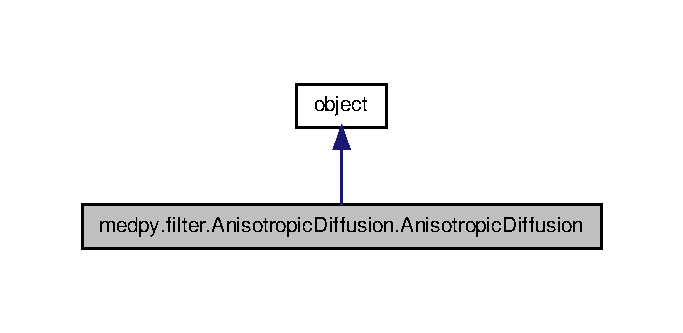
\includegraphics[width=328pt]{classmedpy_1_1filter_1_1AnisotropicDiffusion_1_1AnisotropicDiffusion__inherit__graph}
\end{center}
\end{figure}


Collaboration diagram for medpy.filter.AnisotropicDiffusion.AnisotropicDiffusion:\nopagebreak
\begin{figure}[H]
\begin{center}
\leavevmode
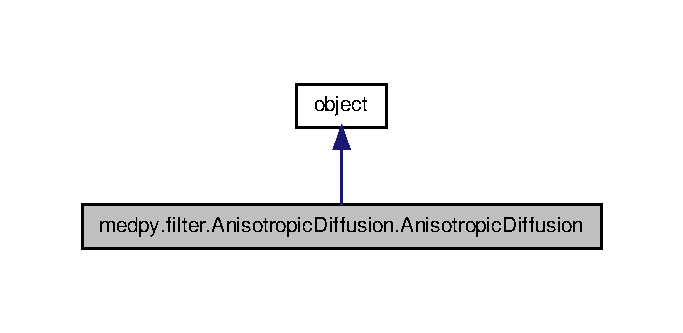
\includegraphics[width=328pt]{classmedpy_1_1filter_1_1AnisotropicDiffusion_1_1AnisotropicDiffusion__coll__graph}
\end{center}
\end{figure}
\subsection*{Public Member Functions}
\begin{DoxyCompactItemize}
\item 
\hypertarget{classmedpy_1_1filter_1_1AnisotropicDiffusion_1_1AnisotropicDiffusion_a44c36411bf89fa4363f8530fd1c95e08}{
def {\bfseries \_\-\_\-init\_\-\_\-}}
\label{classmedpy_1_1filter_1_1AnisotropicDiffusion_1_1AnisotropicDiffusion_a44c36411bf89fa4363f8530fd1c95e08}

\item 
\hypertarget{classmedpy_1_1filter_1_1AnisotropicDiffusion_1_1AnisotropicDiffusion_a0570346712d774d5924136d2db5b1900}{
def {\bfseries anisotropic\_\-diffusion}}
\label{classmedpy_1_1filter_1_1AnisotropicDiffusion_1_1AnisotropicDiffusion_a0570346712d774d5924136d2db5b1900}

\end{DoxyCompactItemize}


\subsection{Detailed Description}


Definition at line 24 of file AnisotropicDiffusion.py.



The documentation for this class was generated from the following file:\begin{DoxyCompactItemize}
\item 
/home/omaier/Programming/Python/medpy/src/medpy/filter/AnisotropicDiffusion.py\end{DoxyCompactItemize}

\hypertarget{classmedpy_1_1core_1_1exceptions_1_1ArgumentError}{
\section{medpy.core.exceptions.ArgumentError Class Reference}
\label{classmedpy_1_1core_1_1exceptions_1_1ArgumentError}\index{medpy::core::exceptions::ArgumentError@{medpy::core::exceptions::ArgumentError}}
}


Thrown by an application when an invalid command line argument has been supplied.  




Inheritance diagram for medpy.core.exceptions.ArgumentError:\nopagebreak
\begin{figure}[H]
\begin{center}
\leavevmode
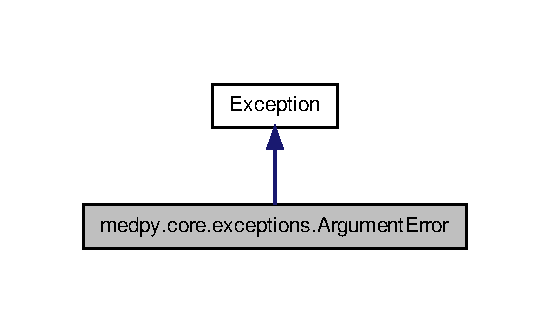
\includegraphics[width=264pt]{classmedpy_1_1core_1_1exceptions_1_1ArgumentError__inherit__graph}
\end{center}
\end{figure}


Collaboration diagram for medpy.core.exceptions.ArgumentError:\nopagebreak
\begin{figure}[H]
\begin{center}
\leavevmode
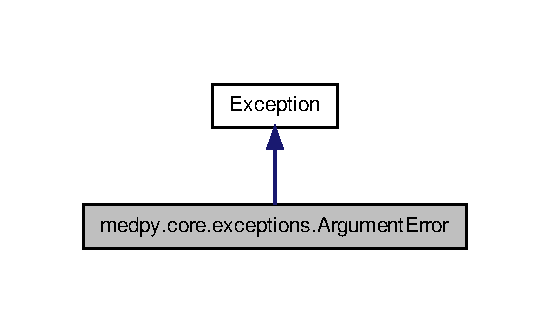
\includegraphics[width=264pt]{classmedpy_1_1core_1_1exceptions_1_1ArgumentError__coll__graph}
\end{center}
\end{figure}


\subsection{Detailed Description}
Thrown by an application when an invalid command line argument has been supplied. 

Definition at line 28 of file exceptions.py.



The documentation for this class was generated from the following file:\begin{DoxyCompactItemize}
\item 
/home/loli/Programming/Python/MedPy/src/medpy/core/exceptions.py\end{DoxyCompactItemize}

\hypertarget{classException}{
\section{Exception Class Reference}
\label{classException}\index{Exception@{Exception}}
}


Inheritance diagram for Exception:\nopagebreak
\begin{figure}[H]
\begin{center}
\leavevmode
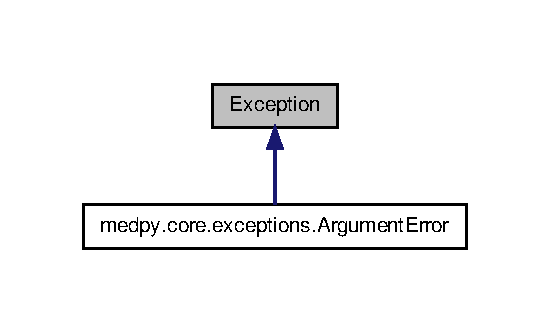
\includegraphics[width=264pt]{classException__inherit__graph}
\end{center}
\end{figure}


The documentation for this class was generated from the following file:\begin{DoxyCompactItemize}
\item 
/home/loli/Programming/Python/MedPy/src/medpy/core/exceptions.py\end{DoxyCompactItemize}

\hypertarget{classmedpy_1_1core_1_1Logger_1_1Logger}{
\section{medpy.core.Logger.Logger Class Reference}
\label{classmedpy_1_1core_1_1Logger_1_1Logger}\index{medpy::core::Logger::Logger@{medpy::core::Logger::Logger}}
}


This singleton class represents an object that can be used by all applications and classes.  




Inheritance diagram for medpy.core.Logger.Logger:\nopagebreak
\begin{figure}[H]
\begin{center}
\leavevmode
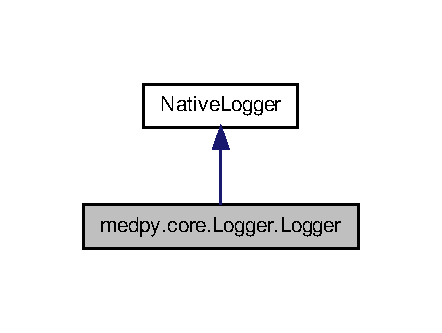
\includegraphics[width=212pt]{classmedpy_1_1core_1_1Logger_1_1Logger__inherit__graph}
\end{center}
\end{figure}


Collaboration diagram for medpy.core.Logger.Logger:\nopagebreak
\begin{figure}[H]
\begin{center}
\leavevmode
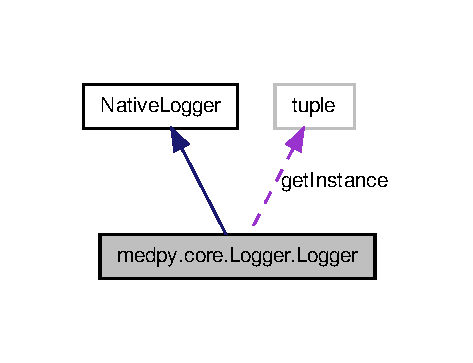
\includegraphics[width=227pt]{classmedpy_1_1core_1_1Logger_1_1Logger__coll__graph}
\end{center}
\end{figure}
\subsection*{Classes}
\begin{DoxyCompactItemize}
\item 
class \hyperlink{classmedpy_1_1core_1_1Logger_1_1Logger_1_1LoggerHelper}{LoggerHelper}
\begin{DoxyCompactList}\small\item\em A helper class which performs the actual initialization. \end{DoxyCompactList}\end{DoxyCompactItemize}
\subsection*{Public Member Functions}
\begin{DoxyCompactItemize}
\item 
\hypertarget{classmedpy_1_1core_1_1Logger_1_1Logger_a8fdfdb7972f6ca4f3b20e98985988bc7}{
def {\bfseries \_\-\_\-init\_\-\_\-}}
\label{classmedpy_1_1core_1_1Logger_1_1Logger_a8fdfdb7972f6ca4f3b20e98985988bc7}

\item 
def \hyperlink{classmedpy_1_1core_1_1Logger_1_1Logger_a9b4ca5d9e5d84d5da1ebda4929c3d757}{setHandler}
\begin{DoxyCompactList}\small\item\em Replaces the current handler with a new one. \end{DoxyCompactList}\item 
\hypertarget{classmedpy_1_1core_1_1Logger_1_1Logger_a7ef3cbfa57e61d02882e586ff7baa176}{
def \hyperlink{classmedpy_1_1core_1_1Logger_1_1Logger_a7ef3cbfa57e61d02882e586ff7baa176}{setLevel}}
\label{classmedpy_1_1core_1_1Logger_1_1Logger_a7ef3cbfa57e61d02882e586ff7baa176}

\begin{DoxyCompactList}\small\item\em Overrides the parent method to adapt the formatting string to the level. \end{DoxyCompactList}\end{DoxyCompactItemize}
\subsection*{Static Public Attributes}
\begin{DoxyCompactItemize}
\item 
\hypertarget{classmedpy_1_1core_1_1Logger_1_1Logger_ae169695a25c1a25f4929d03eb5ff016b}{
tuple {\bfseries getInstance} = \hyperlink{classmedpy_1_1core_1_1Logger_1_1Logger_1_1LoggerHelper}{LoggerHelper}()}
\label{classmedpy_1_1core_1_1Logger_1_1Logger_ae169695a25c1a25f4929d03eb5ff016b}

\end{DoxyCompactItemize}
\subsection*{Static Private Attributes}
\begin{DoxyCompactItemize}
\item 
\hypertarget{classmedpy_1_1core_1_1Logger_1_1Logger_af48b52980156fd81d4297cf243204a1e}{
{\bfseries \_\-instance} = None}
\label{classmedpy_1_1core_1_1Logger_1_1Logger_af48b52980156fd81d4297cf243204a1e}

\item 
\hypertarget{classmedpy_1_1core_1_1Logger_1_1Logger_a82158993b8453bc1b8881f5e92a413ff}{
{\bfseries \_\-handler} = None}
\label{classmedpy_1_1core_1_1Logger_1_1Logger_a82158993b8453bc1b8881f5e92a413ff}

\end{DoxyCompactItemize}


\subsection{Detailed Description}
This singleton class represents an object that can be used by all applications and classes. 

Definition at line 34 of file Logger.py.



\subsection{Member Function Documentation}
\hypertarget{classmedpy_1_1core_1_1Logger_1_1Logger_a9b4ca5d9e5d84d5da1ebda4929c3d757}{
\index{medpy::core::Logger::Logger@{medpy::core::Logger::Logger}!setHandler@{setHandler}}
\index{setHandler@{setHandler}!medpy::core::Logger::Logger@{medpy::core::Logger::Logger}}
\subsubsection[{setHandler}]{\setlength{\rightskip}{0pt plus 5cm}def medpy.core.Logger.Logger.setHandler (
\begin{DoxyParamCaption}
\item[{}]{self, }
\item[{}]{hdlr}
\end{DoxyParamCaption}
)}}
\label{classmedpy_1_1core_1_1Logger_1_1Logger_a9b4ca5d9e5d84d5da1ebda4929c3d757}


Replaces the current handler with a new one. 

If none should be replaces, but just one added, use the parent classes addHandler() method. 

Definition at line 76 of file Logger.py.



The documentation for this class was generated from the following file:\begin{DoxyCompactItemize}
\item 
/home/loli/Programming/Python/MedPy/src/medpy/core/Logger.py\end{DoxyCompactItemize}

\hypertarget{classmedpy_1_1core_1_1Logger_1_1Logger_1_1LoggerHelper}{
\section{medpy.core.Logger.Logger.LoggerHelper Class Reference}
\label{classmedpy_1_1core_1_1Logger_1_1Logger_1_1LoggerHelper}\index{medpy::core::Logger::Logger::LoggerHelper@{medpy::core::Logger::Logger::LoggerHelper}}
}


A helper class which performs the actual initialization.  




Inheritance diagram for medpy.core.Logger.Logger.LoggerHelper:\nopagebreak
\begin{figure}[H]
\begin{center}
\leavevmode
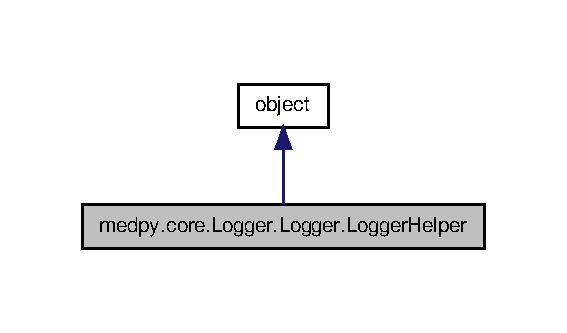
\includegraphics[width=272pt]{classmedpy_1_1core_1_1Logger_1_1Logger_1_1LoggerHelper__inherit__graph}
\end{center}
\end{figure}


Collaboration diagram for medpy.core.Logger.Logger.LoggerHelper:\nopagebreak
\begin{figure}[H]
\begin{center}
\leavevmode
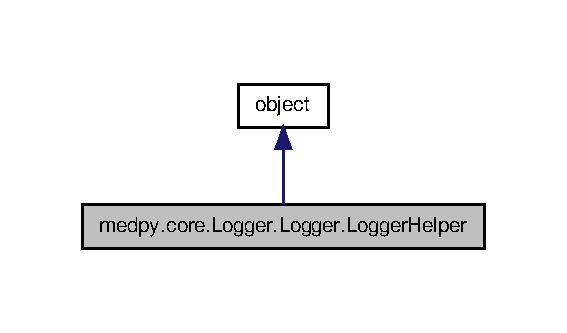
\includegraphics[width=272pt]{classmedpy_1_1core_1_1Logger_1_1Logger_1_1LoggerHelper__coll__graph}
\end{center}
\end{figure}
\subsection*{Public Member Functions}
\begin{DoxyCompactItemize}
\item 
\hypertarget{classmedpy_1_1core_1_1Logger_1_1Logger_1_1LoggerHelper_aea5d63b929cd6340bc6f8f249956e44b}{
def {\bfseries \_\-\_\-call\_\-\_\-}}
\label{classmedpy_1_1core_1_1Logger_1_1Logger_1_1LoggerHelper_aea5d63b929cd6340bc6f8f249956e44b}

\end{DoxyCompactItemize}


\subsection{Detailed Description}
A helper class which performs the actual initialization. 

Definition at line 40 of file Logger.py.



The documentation for this class was generated from the following file:\begin{DoxyCompactItemize}
\item 
/home/loli/Programming/Python/MedPy/src/medpy/core/Logger.py\end{DoxyCompactItemize}

\hypertarget{classNativeLogger}{
\section{NativeLogger Class Reference}
\label{classNativeLogger}\index{NativeLogger@{NativeLogger}}
}


Inheritance diagram for NativeLogger:\nopagebreak
\begin{figure}[H]
\begin{center}
\leavevmode
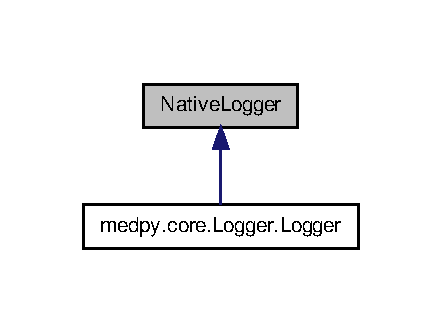
\includegraphics[width=212pt]{classNativeLogger__inherit__graph}
\end{center}
\end{figure}


The documentation for this class was generated from the following file:\begin{DoxyCompactItemize}
\item 
/home/loli/Programming/Python/MedPy/src/medpy/core/Logger.py\end{DoxyCompactItemize}

\hypertarget{classobject}{
\section{object Class Reference}
\label{classobject}\index{object@{object}}
}


Inheritance diagram for object:\nopagebreak
\begin{figure}[H]
\begin{center}
\leavevmode
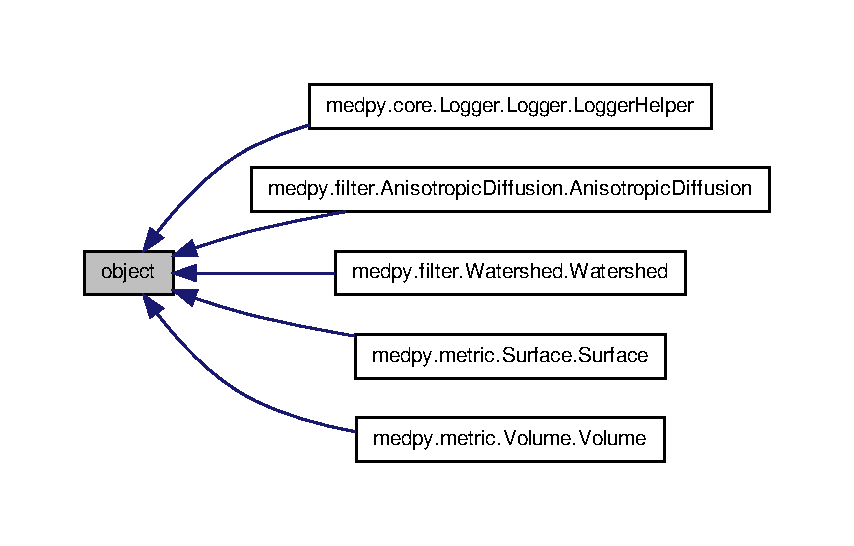
\includegraphics[width=400pt]{classobject__inherit__graph}
\end{center}
\end{figure}


The documentation for this class was generated from the following file:\begin{DoxyCompactItemize}
\item 
/home/omaier/Programming/Python/medpy/src/medpy/filter/AnisotropicDiffusion.py\end{DoxyCompactItemize}

\hypertarget{classmedpy_1_1metric_1_1Surface_1_1Surface}{
\section{medpy.metric.Surface.Surface Class Reference}
\label{classmedpy_1_1metric_1_1Surface_1_1Surface}\index{medpy::metric::Surface::Surface@{medpy::metric::Surface::Surface}}
}


Computes different surface metrics between two 3D-\/images contain each an object.  




Inheritance diagram for medpy.metric.Surface.Surface:\nopagebreak
\begin{figure}[H]
\begin{center}
\leavevmode
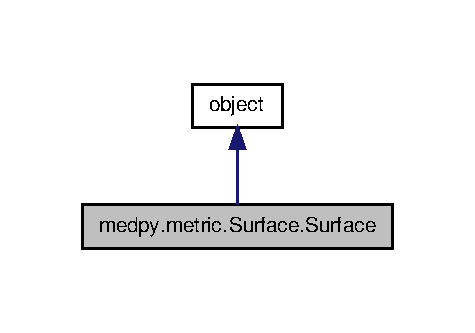
\includegraphics[width=228pt]{classmedpy_1_1metric_1_1Surface_1_1Surface__inherit__graph}
\end{center}
\end{figure}


Collaboration diagram for medpy.metric.Surface.Surface:\nopagebreak
\begin{figure}[H]
\begin{center}
\leavevmode
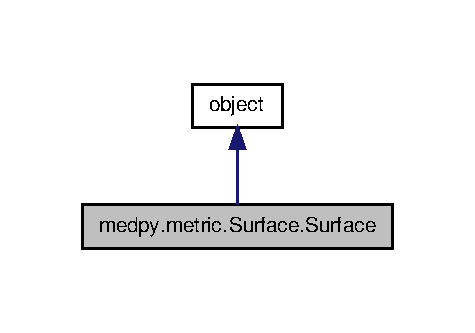
\includegraphics[width=228pt]{classmedpy_1_1metric_1_1Surface_1_1Surface__coll__graph}
\end{center}
\end{figure}
\subsection*{Public Member Functions}
\begin{DoxyCompactItemize}
\item 
def \hyperlink{classmedpy_1_1metric_1_1Surface_1_1Surface_ab5851eb70bda096a86fb6716060167b7}{\_\-\_\-init\_\-\_\-}
\begin{DoxyCompactList}\small\item\em Initialize the class with two binary images, each containing a single object. \end{DoxyCompactList}\item 
def \hyperlink{classmedpy_1_1metric_1_1Surface_1_1Surface_a9cdf888536ae9f7ed0576fac57ac77c2}{GetMaximumSymmetricSurfaceDistance}
\begin{DoxyCompactList}\small\item\em Computes the maximum symmetric surface distance, also known as Hausdorff distance, between the two objects surfaces. \end{DoxyCompactList}\item 
def \hyperlink{classmedpy_1_1metric_1_1Surface_1_1Surface_a0d6bcf9373cb1a2f9f04ca28b8d208f9}{GetRootMeanSquareSymmetricSurfaceDistance}
\begin{DoxyCompactList}\small\item\em Computes the root mean square symmetric surface distance between the two objects surfaces. \end{DoxyCompactList}\item 
def \hyperlink{classmedpy_1_1metric_1_1Surface_1_1Surface_a1f1c1e69dd67604384b5aa5656551452}{GetAverageSymmetricSurfaceDistance}
\begin{DoxyCompactList}\small\item\em Computes the average symmetric surface distance between the two objects surfaces. \end{DoxyCompactList}\item 
def \hyperlink{classmedpy_1_1metric_1_1Surface_1_1Surface_a4d61287dc4a1f0caa0571c68ec1a5cb7}{GetMaskReferenceNn}
\item 
def \hyperlink{classmedpy_1_1metric_1_1Surface_1_1Surface_a1ae1504a6292716aa10a53cf98d61b81}{GetReferenceMaskNn}
\item 
def \hyperlink{classmedpy_1_1metric_1_1Surface_1_1Surface_a70d79edef12225a428163cea7dffcf0d}{GetMaskEdgePoints}
\item 
def \hyperlink{classmedpy_1_1metric_1_1Surface_1_1Surface_af373420f97720cbd0680cd7a23f18417}{GetReferenceEdgePoints}
\end{DoxyCompactItemize}
\paragraph*{}
\begin{DoxyCompactItemize}
\item 
def \hyperlink{classmedpy_1_1metric_1_1Surface_1_1Surface_a7816a65c3be7f869e47a6094e456342e}{ComputeContour}
\begin{DoxyCompactList}\small\item\em Uses a 18-\/neighbourhood filter to create an edge image of the input object. \end{DoxyCompactList}\end{DoxyCompactItemize}



\subsection{Detailed Description}
Computes different surface metrics between two 3D-\/images contain each an object. 

The surface of the objects is computed using a 18-\/neighbourhood edge detection. The distance metrics are computed over all points of the surfaces using the nearest neighbour approach. Beside this provides a number of statistics of the two images.

During the initialization the edge detection is run for both images, taking up to 5 min (on 512$^\wedge$3 images). The first call to one of the metric measures triggers the computation of the nearest neighbours, taking up to 7 minutes (based on 250.000 edge point for each of the objects, which corresponds to a typical liver mask). All subsequent calls to one of the metrics measures can be expected be in the sub-\/millisecond area.

Metrics defined in: Heimann, T.; van Ginneken, B.; Styner, M.A.; Arzhaeva, Y.; Aurich, V.; Bauer, C.; Beck, A.; Becker, C.; Beichel, R.; Bekes, G.; Bello, F.; Binnig, G.; Bischof, H.; Bornik, A.; Cashman, P.; Ying Chi; Cordova, A.; Dawant, B.M.; Fidrich, M.; Furst, J.D.; Furukawa, D.; Grenacher, L.; Hornegger, J.; Kainmuller, D.; Kitney, R.I.; Kobatake, H.; Lamecker, H.; Lange, T.; Jeongjin Lee; Lennon, B.; Rui Li; Senhu Li; Meinzer, H.-\/P.; Nemeth, G.; Raicu, D.S.; Rau, A.-\/M.; van Rikxoort, E.M.; Rousson, M.; Rusko, L.; Saddi, K.A.; Schmidt, G.; Seghers, D.; Shimizu, A.; Slagmolen, P.; Sorantin, E.; Soza, G.; Susomboon, R.; Waite, J.M.; Wimmer, A.; Wolf, I.; , \char`\"{}Comparison and Evaluation of Methods for Liver Segmentation From CT Datasets,\char`\"{} Medical Imaging, IEEE Transactions on , vol.28, no.8, pp.1251-\/1265, Aug. 2009 doi: 10.1109/TMI.2009.2013851 \begin{DoxyVerb}The edge points of the mask object.\end{DoxyVerb}
 

Definition at line 44 of file Surface.py.



\subsection{Constructor \& Destructor Documentation}
\hypertarget{classmedpy_1_1metric_1_1Surface_1_1Surface_ab5851eb70bda096a86fb6716060167b7}{
\index{medpy::metric::Surface::Surface@{medpy::metric::Surface::Surface}!\_\-\_\-init\_\-\_\-@{\_\-\_\-init\_\-\_\-}}
\index{\_\-\_\-init\_\-\_\-@{\_\-\_\-init\_\-\_\-}!medpy::metric::Surface::Surface@{medpy::metric::Surface::Surface}}
\subsubsection[{\_\-\_\-init\_\-\_\-}]{\setlength{\rightskip}{0pt plus 5cm}def medpy.metric.Surface.Surface.\_\-\_\-init\_\-\_\- (
\begin{DoxyParamCaption}
\item[{}]{self, }
\item[{}]{mask, }
\item[{}]{reference, }
\item[{}]{physical\_\-voxel\_\-spacing = {\ttfamily \mbox{[}1}, }
\item[{}]{mask\_\-offset = {\ttfamily \mbox{[}0}, }
\item[{}]{reference\_\-offset = {\ttfamily \mbox{[}0}}
\end{DoxyParamCaption}
)}}
\label{classmedpy_1_1metric_1_1Surface_1_1Surface_ab5851eb70bda096a86fb6716060167b7}


Initialize the class with two binary images, each containing a single object. 

Assumes the input to be a representation of a 3D image, that fits one of the following formats: 1. all 0 values denoting background, all others the foreground/object 2. all False values denoting the background, all others the foreground/object The first image passed is referred to as 'mask', the second as 'reference'. This is only important for some metrics that are not symmetric (and therefore not really metrics). 
\begin{DoxyParams}{Parameters}
{\em mask,:} & binary mask as an scipy array (3D image) \\
\hline
{\em reference,:} & binary reference as an scipy array (3D image) \\
\hline
{\em physical\_\-voxel\_\-spacing,:} & The physical voxel spacing of the two images (must be the same for both) \\
\hline
{\em mask\_\-offset,:} & offset of the mask array to 0,0,0-\/origin \\
\hline
{\em reference\_\-offset,:} & offset of the reference array to 0,0,0-\/origin \\
\hline
\end{DoxyParams}


Definition at line 74 of file Surface.py.



\subsection{Member Function Documentation}
\hypertarget{classmedpy_1_1metric_1_1Surface_1_1Surface_a7816a65c3be7f869e47a6094e456342e}{
\index{medpy::metric::Surface::Surface@{medpy::metric::Surface::Surface}!ComputeContour@{ComputeContour}}
\index{ComputeContour@{ComputeContour}!medpy::metric::Surface::Surface@{medpy::metric::Surface::Surface}}
\subsubsection[{ComputeContour}]{\setlength{\rightskip}{0pt plus 5cm}def medpy.metric.Surface.Surface.ComputeContour (
\begin{DoxyParamCaption}
\item[{}]{array}
\end{DoxyParamCaption}
)}}
\label{classmedpy_1_1metric_1_1Surface_1_1Surface_a7816a65c3be7f869e47a6094e456342e}


Uses a 18-\/neighbourhood filter to create an edge image of the input object. 

Assumes the input to be a representation of a 3D image, that fits one of the following formats: 1. all 0 values denoting background, all others the foreground/object 2. all False values denoting the background, all others the foreground/object The area outside the array is assumed to contain background voxels. The method does not ensure that the object voxels are actually connected, this is silently assumed.


\begin{DoxyParams}{Parameters}
{\em array,:} & a numpy array with only 0/N0\} or False/True values. \\
\hline
\end{DoxyParams}
\begin{DoxyReturn}{Returns}
: a boolean numpy array with the input objects edges 
\end{DoxyReturn}


Definition at line 295 of file Surface.py.

\hypertarget{classmedpy_1_1metric_1_1Surface_1_1Surface_a1f1c1e69dd67604384b5aa5656551452}{
\index{medpy::metric::Surface::Surface@{medpy::metric::Surface::Surface}!GetAverageSymmetricSurfaceDistance@{GetAverageSymmetricSurfaceDistance}}
\index{GetAverageSymmetricSurfaceDistance@{GetAverageSymmetricSurfaceDistance}!medpy::metric::Surface::Surface@{medpy::metric::Surface::Surface}}
\subsubsection[{GetAverageSymmetricSurfaceDistance}]{\setlength{\rightskip}{0pt plus 5cm}def medpy.metric.Surface.Surface.GetAverageSymmetricSurfaceDistance (
\begin{DoxyParamCaption}
\item[{}]{self}
\end{DoxyParamCaption}
)}}
\label{classmedpy_1_1metric_1_1Surface_1_1Surface_a1f1c1e69dd67604384b5aa5656551452}


Computes the average symmetric surface distance between the two objects surfaces. 

\begin{DoxyReturn}{Returns}
: average symmetric surface distance in millimeters
\end{DoxyReturn}
For a perfect segmentation this distance is 0.

Metric definition: Let $S(A)$ denote the set of surface voxels of $A$. The shortest distance of an arbitrary voxel $v$ to $S(A)$ is defined as: \[ d(v,S(A)) = \min_{s_A\in S(A)} ||v-s_A|| \] where $||.||$ denotes the Euclidean distance. The average symmetric surface distance is then given by: \[ ASD(A,B) = \frac{1}{|S(A)|+|S(B)|} \left( \sum_{s_A\in S(A)} d(s_A,S(B)) + \sum_{s_B\in S(B)} d(s_B,S(A)) \right) \] 

Definition at line 218 of file Surface.py.

\hypertarget{classmedpy_1_1metric_1_1Surface_1_1Surface_a70d79edef12225a428163cea7dffcf0d}{
\index{medpy::metric::Surface::Surface@{medpy::metric::Surface::Surface}!GetMaskEdgePoints@{GetMaskEdgePoints}}
\index{GetMaskEdgePoints@{GetMaskEdgePoints}!medpy::metric::Surface::Surface@{medpy::metric::Surface::Surface}}
\subsubsection[{GetMaskEdgePoints}]{\setlength{\rightskip}{0pt plus 5cm}def medpy.metric.Surface.Surface.GetMaskEdgePoints (
\begin{DoxyParamCaption}
\item[{}]{self}
\end{DoxyParamCaption}
)}}
\label{classmedpy_1_1metric_1_1Surface_1_1Surface_a70d79edef12225a428163cea7dffcf0d}
\begin{DoxyReturn}{Returns}
: The edge points of the mask object. 
\end{DoxyReturn}


Definition at line 270 of file Surface.py.

\hypertarget{classmedpy_1_1metric_1_1Surface_1_1Surface_a4d61287dc4a1f0caa0571c68ec1a5cb7}{
\index{medpy::metric::Surface::Surface@{medpy::metric::Surface::Surface}!GetMaskReferenceNn@{GetMaskReferenceNn}}
\index{GetMaskReferenceNn@{GetMaskReferenceNn}!medpy::metric::Surface::Surface@{medpy::metric::Surface::Surface}}
\subsubsection[{GetMaskReferenceNn}]{\setlength{\rightskip}{0pt plus 5cm}def medpy.metric.Surface.Surface.GetMaskReferenceNn (
\begin{DoxyParamCaption}
\item[{}]{self}
\end{DoxyParamCaption}
)}}
\label{classmedpy_1_1metric_1_1Surface_1_1Surface_a4d61287dc4a1f0caa0571c68ec1a5cb7}
\begin{DoxyReturn}{Returns}
: The distances of the nearest neighbours of all mask edge points to all reference edge points. 
\end{DoxyReturn}


Definition at line 239 of file Surface.py.

\hypertarget{classmedpy_1_1metric_1_1Surface_1_1Surface_a9cdf888536ae9f7ed0576fac57ac77c2}{
\index{medpy::metric::Surface::Surface@{medpy::metric::Surface::Surface}!GetMaximumSymmetricSurfaceDistance@{GetMaximumSymmetricSurfaceDistance}}
\index{GetMaximumSymmetricSurfaceDistance@{GetMaximumSymmetricSurfaceDistance}!medpy::metric::Surface::Surface@{medpy::metric::Surface::Surface}}
\subsubsection[{GetMaximumSymmetricSurfaceDistance}]{\setlength{\rightskip}{0pt plus 5cm}def medpy.metric.Surface.Surface.GetMaximumSymmetricSurfaceDistance (
\begin{DoxyParamCaption}
\item[{}]{self}
\end{DoxyParamCaption}
)}}
\label{classmedpy_1_1metric_1_1Surface_1_1Surface_a9cdf888536ae9f7ed0576fac57ac77c2}


Computes the maximum symmetric surface distance, also known as Hausdorff distance, between the two objects surfaces. 

\begin{DoxyReturn}{Returns}
: the maximum symmetric surface distance in millimeters
\end{DoxyReturn}
For a perfect segmentation this distance is 0. This metric is sensitive to outliers and returns the true maximum error.

Metric definition: Let $S(A)$ denote the set of surface voxels of $A$. The shortest distance of an arbitrary voxel $v$ to $S(A)$ is defined as: \[ d(v,S(A)) = \min_{s_A\in S(A)} ||v-s_A|| \] where $||.||$ denotes the Euclidean distance. The maximum symmetric surface distance is then given by: \[ MSD(A,B) = \max \left\{ \max_{s_A\in S(A)} d(s_A,S(B)), \max_{s_B\in S(B)} d(s_B,S(A)), \right\} \] 

Definition at line 133 of file Surface.py.

\hypertarget{classmedpy_1_1metric_1_1Surface_1_1Surface_af373420f97720cbd0680cd7a23f18417}{
\index{medpy::metric::Surface::Surface@{medpy::metric::Surface::Surface}!GetReferenceEdgePoints@{GetReferenceEdgePoints}}
\index{GetReferenceEdgePoints@{GetReferenceEdgePoints}!medpy::metric::Surface::Surface@{medpy::metric::Surface::Surface}}
\subsubsection[{GetReferenceEdgePoints}]{\setlength{\rightskip}{0pt plus 5cm}def medpy.metric.Surface.Surface.GetReferenceEdgePoints (
\begin{DoxyParamCaption}
\item[{}]{self}
\end{DoxyParamCaption}
)}}
\label{classmedpy_1_1metric_1_1Surface_1_1Surface_af373420f97720cbd0680cd7a23f18417}
\begin{DoxyReturn}{Returns}
: The edge points of the reference object. 
\end{DoxyReturn}


Definition at line 277 of file Surface.py.

\hypertarget{classmedpy_1_1metric_1_1Surface_1_1Surface_a1ae1504a6292716aa10a53cf98d61b81}{
\index{medpy::metric::Surface::Surface@{medpy::metric::Surface::Surface}!GetReferenceMaskNn@{GetReferenceMaskNn}}
\index{GetReferenceMaskNn@{GetReferenceMaskNn}!medpy::metric::Surface::Surface@{medpy::metric::Surface::Surface}}
\subsubsection[{GetReferenceMaskNn}]{\setlength{\rightskip}{0pt plus 5cm}def medpy.metric.Surface.Surface.GetReferenceMaskNn (
\begin{DoxyParamCaption}
\item[{}]{self}
\end{DoxyParamCaption}
)}}
\label{classmedpy_1_1metric_1_1Surface_1_1Surface_a1ae1504a6292716aa10a53cf98d61b81}
\begin{DoxyReturn}{Returns}
: The distances of the nearest neighbours of all reference edge points to all mask edge points.
\end{DoxyReturn}
The underlying algorithm used for the scipy.spatial.KDTree implementation is based on: Sunil Arya, David M. Mount, Nathan S. Netanyahu, Ruth Silverman, and Angela Y. Wu. 1998. An optimal algorithm for approximate nearest neighbor searching fixed dimensions. J. ACM 45, 6 (November 1998), 891-\/923 

Definition at line 257 of file Surface.py.

\hypertarget{classmedpy_1_1metric_1_1Surface_1_1Surface_a0d6bcf9373cb1a2f9f04ca28b8d208f9}{
\index{medpy::metric::Surface::Surface@{medpy::metric::Surface::Surface}!GetRootMeanSquareSymmetricSurfaceDistance@{GetRootMeanSquareSymmetricSurfaceDistance}}
\index{GetRootMeanSquareSymmetricSurfaceDistance@{GetRootMeanSquareSymmetricSurfaceDistance}!medpy::metric::Surface::Surface@{medpy::metric::Surface::Surface}}
\subsubsection[{GetRootMeanSquareSymmetricSurfaceDistance}]{\setlength{\rightskip}{0pt plus 5cm}def medpy.metric.Surface.Surface.GetRootMeanSquareSymmetricSurfaceDistance (
\begin{DoxyParamCaption}
\item[{}]{self}
\end{DoxyParamCaption}
)}}
\label{classmedpy_1_1metric_1_1Surface_1_1Surface_a0d6bcf9373cb1a2f9f04ca28b8d208f9}


Computes the root mean square symmetric surface distance between the two objects surfaces. 

\begin{DoxyReturn}{Returns}
: root mean square symmetric surface distance in millimeters
\end{DoxyReturn}
For a perfect segmentation this distance is 0. This metric punishes large deviations from the true contour stronger than the average symmetric surface distance.

Metric definition: Let $S(A)$ denote the set of surface voxels of $A$. The shortest distance of an arbitrary voxel $v$ to $S(A)$ is defined as: \[ d(v,S(A)) = \min_{s_A\in S(A)} ||v-s_A|| \] where $||.||$ denotes the Euclidean distance. The root mean square symmetric surface distance is then given by: \[ RMSD(A,B) = \sqrt{\frac{1}{|S(A)|+|S(B)|}} \times \sqrt{ \sum_{s_A\in S(A)} d^2(s_A,S(B)) + \sum_{s_B\in S(B)} d^2(s_B,S(A)) } \] 

Definition at line 171 of file Surface.py.



The documentation for this class was generated from the following file:\begin{DoxyCompactItemize}
\item 
/home/omaier/Programming/Python/medpy/src/medpy/metric/Surface.py\end{DoxyCompactItemize}

\hypertarget{classunittest_1_1TestCase}{
\section{TestCase Class Reference}
\label{classunittest_1_1TestCase}\index{unittest::TestCase@{unittest::TestCase}}
}


Inheritance diagram for TestCase:\nopagebreak
\begin{figure}[H]
\begin{center}
\leavevmode
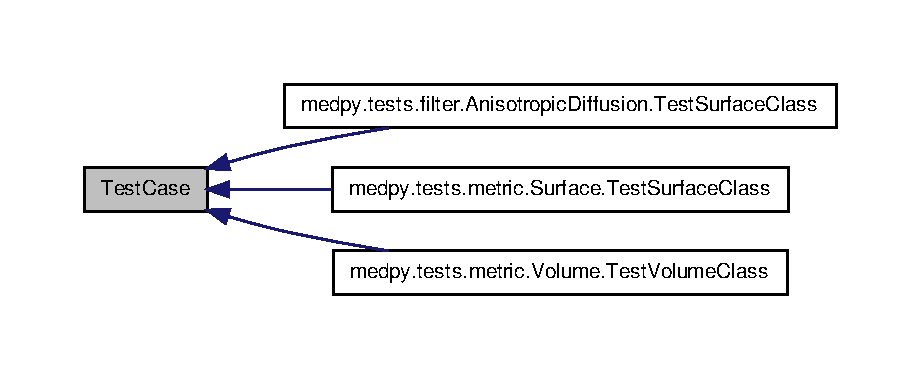
\includegraphics[width=400pt]{classunittest_1_1TestCase__inherit__graph}
\end{center}
\end{figure}


The documentation for this class was generated from the following file:\begin{DoxyCompactItemize}
\item 
/home/loli/Programming/Python/MedPy/src/medpy/tests/metric/Surface.py\end{DoxyCompactItemize}

\hypertarget{classmedpy_1_1tests_1_1filter_1_1AnisotropicDiffusion_1_1TestSurfaceClass}{
\section{medpy.tests.filter.AnisotropicDiffusion.TestSurfaceClass Class Reference}
\label{classmedpy_1_1tests_1_1filter_1_1AnisotropicDiffusion_1_1TestSurfaceClass}\index{medpy::tests::filter::AnisotropicDiffusion::TestSurfaceClass@{medpy::tests::filter::AnisotropicDiffusion::TestSurfaceClass}}
}


Inheritance diagram for medpy.tests.filter.AnisotropicDiffusion.TestSurfaceClass:\nopagebreak
\begin{figure}[H]
\begin{center}
\leavevmode
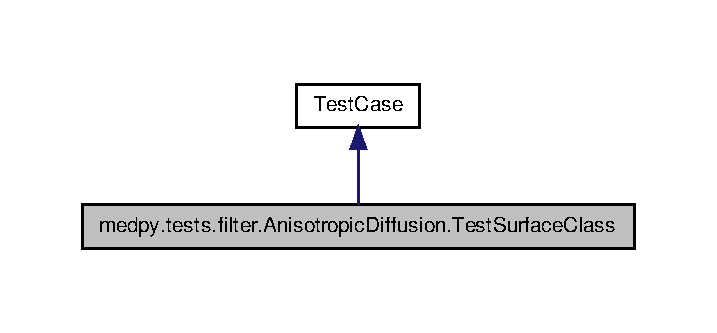
\includegraphics[width=344pt]{classmedpy_1_1tests_1_1filter_1_1AnisotropicDiffusion_1_1TestSurfaceClass__inherit__graph}
\end{center}
\end{figure}


Collaboration diagram for medpy.tests.filter.AnisotropicDiffusion.TestSurfaceClass:\nopagebreak
\begin{figure}[H]
\begin{center}
\leavevmode
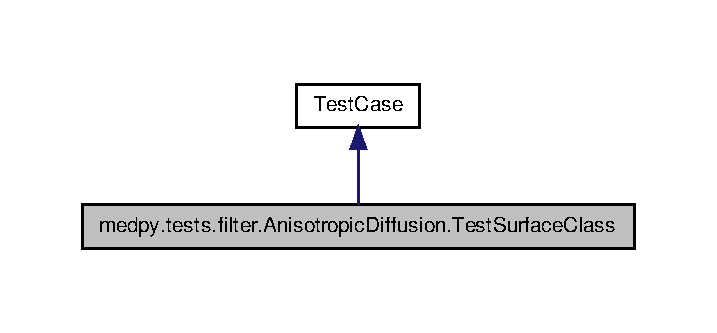
\includegraphics[width=344pt]{classmedpy_1_1tests_1_1filter_1_1AnisotropicDiffusion_1_1TestSurfaceClass__coll__graph}
\end{center}
\end{figure}
\subsection*{Public Member Functions}
\begin{DoxyCompactItemize}
\item 
\hypertarget{classmedpy_1_1tests_1_1filter_1_1AnisotropicDiffusion_1_1TestSurfaceClass_ae82f9cb1e824e5bdfe4447c3a1abb3ae}{
def {\bfseries test\_\-diffusion}}
\label{classmedpy_1_1tests_1_1filter_1_1AnisotropicDiffusion_1_1TestSurfaceClass_ae82f9cb1e824e5bdfe4447c3a1abb3ae}

\end{DoxyCompactItemize}


\subsection{Detailed Description}


Definition at line 23 of file AnisotropicDiffusion.py.



The documentation for this class was generated from the following file:\begin{DoxyCompactItemize}
\item 
/home/loli/Programming/Python/MedPy/src/medpy/tests/filter/AnisotropicDiffusion.py\end{DoxyCompactItemize}

\hypertarget{classmedpy_1_1tests_1_1metric_1_1Surface_1_1TestSurfaceClass}{
\section{medpy.tests.metric.Surface.TestSurfaceClass Class Reference}
\label{classmedpy_1_1tests_1_1metric_1_1Surface_1_1TestSurfaceClass}\index{medpy::tests::metric::Surface::TestSurfaceClass@{medpy::tests::metric::Surface::TestSurfaceClass}}
}


Inheritance diagram for medpy.tests.metric.Surface.TestSurfaceClass:\nopagebreak
\begin{figure}[H]
\begin{center}
\leavevmode
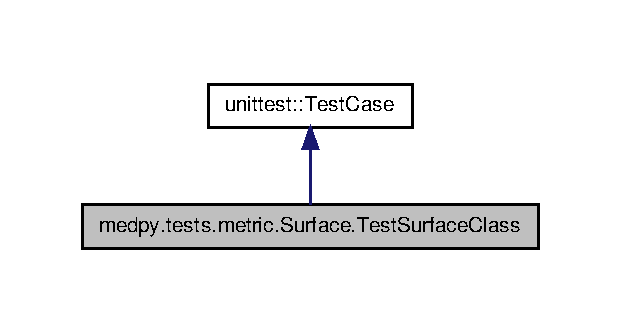
\includegraphics[width=298pt]{classmedpy_1_1tests_1_1metric_1_1Surface_1_1TestSurfaceClass__inherit__graph}
\end{center}
\end{figure}


Collaboration diagram for medpy.tests.metric.Surface.TestSurfaceClass:\nopagebreak
\begin{figure}[H]
\begin{center}
\leavevmode
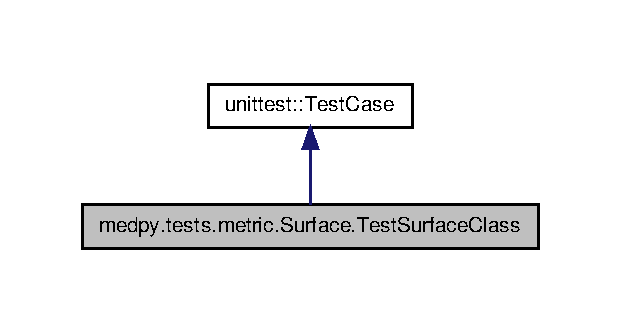
\includegraphics[width=298pt]{classmedpy_1_1tests_1_1metric_1_1Surface_1_1TestSurfaceClass__coll__graph}
\end{center}
\end{figure}
\subsection*{Public Member Functions}
\begin{DoxyCompactItemize}
\item 
\hypertarget{classmedpy_1_1tests_1_1metric_1_1Surface_1_1TestSurfaceClass_a103d826711c85105e3a9b5c51716b254}{
def {\bfseries setUp}}
\label{classmedpy_1_1tests_1_1metric_1_1Surface_1_1TestSurfaceClass_a103d826711c85105e3a9b5c51716b254}

\item 
\hypertarget{classmedpy_1_1tests_1_1metric_1_1Surface_1_1TestSurfaceClass_a5c9954cb59e13a6d026c7a1aae41205f}{
def {\bfseries test\_\-Initialization}}
\label{classmedpy_1_1tests_1_1metric_1_1Surface_1_1TestSurfaceClass_a5c9954cb59e13a6d026c7a1aae41205f}

\item 
\hypertarget{classmedpy_1_1tests_1_1metric_1_1Surface_1_1TestSurfaceClass_a7a6b072bf4d343c9b5aca834f81df880}{
def {\bfseries test\_\-ComputeContour}}
\label{classmedpy_1_1tests_1_1metric_1_1Surface_1_1TestSurfaceClass_a7a6b072bf4d343c9b5aca834f81df880}

\item 
\hypertarget{classmedpy_1_1tests_1_1metric_1_1Surface_1_1TestSurfaceClass_afce12e6ac335ad46e416a67c08b27dee}{
def {\bfseries test\_\-GetMaximumSymmetricSurfaceDistance}}
\label{classmedpy_1_1tests_1_1metric_1_1Surface_1_1TestSurfaceClass_afce12e6ac335ad46e416a67c08b27dee}

\item 
\hypertarget{classmedpy_1_1tests_1_1metric_1_1Surface_1_1TestSurfaceClass_a996ebeccc46c7b81b18a9523ed20a3dc}{
def {\bfseries test\_\-GetAverageSymmetricSurfaceDistance}}
\label{classmedpy_1_1tests_1_1metric_1_1Surface_1_1TestSurfaceClass_a996ebeccc46c7b81b18a9523ed20a3dc}

\item 
\hypertarget{classmedpy_1_1tests_1_1metric_1_1Surface_1_1TestSurfaceClass_a01d1f751f5f0eac65897a844a52dc367}{
def {\bfseries test\_\-GetRootMeanSquareSymmetricSurfaceDistance}}
\label{classmedpy_1_1tests_1_1metric_1_1Surface_1_1TestSurfaceClass_a01d1f751f5f0eac65897a844a52dc367}

\end{DoxyCompactItemize}
\subsection*{Private Attributes}
\begin{DoxyCompactItemize}
\item 
\hypertarget{classmedpy_1_1tests_1_1metric_1_1Surface_1_1TestSurfaceClass_acfe84a31bc62cc25d6fbf8bc845ccbea}{
{\bfseries \_\-imaged1}}
\label{classmedpy_1_1tests_1_1metric_1_1Surface_1_1TestSurfaceClass_acfe84a31bc62cc25d6fbf8bc845ccbea}

\item 
\hypertarget{classmedpy_1_1tests_1_1metric_1_1Surface_1_1TestSurfaceClass_a3a713da5b07b2d172a90962cc4e6e14d}{
{\bfseries \_\-imaged2}}
\label{classmedpy_1_1tests_1_1metric_1_1Surface_1_1TestSurfaceClass_a3a713da5b07b2d172a90962cc4e6e14d}

\item 
\hypertarget{classmedpy_1_1tests_1_1metric_1_1Surface_1_1TestSurfaceClass_a461ec637a55c5e33ff55224fbeba6a2e}{
{\bfseries \_\-imaged3}}
\label{classmedpy_1_1tests_1_1metric_1_1Surface_1_1TestSurfaceClass_a461ec637a55c5e33ff55224fbeba6a2e}

\item 
\hypertarget{classmedpy_1_1tests_1_1metric_1_1Surface_1_1TestSurfaceClass_a16ae600222aca4f6201cc25f89543147}{
{\bfseries \_\-imaged4}}
\label{classmedpy_1_1tests_1_1metric_1_1Surface_1_1TestSurfaceClass_a16ae600222aca4f6201cc25f89543147}

\item 
\hypertarget{classmedpy_1_1tests_1_1metric_1_1Surface_1_1TestSurfaceClass_ae23c90322f0c7fb8b87b8e9753faf3e7}{
{\bfseries \_\-imagedA}}
\label{classmedpy_1_1tests_1_1metric_1_1Surface_1_1TestSurfaceClass_ae23c90322f0c7fb8b87b8e9753faf3e7}

\item 
\hypertarget{classmedpy_1_1tests_1_1metric_1_1Surface_1_1TestSurfaceClass_a9e3a1a65426aac370c8f6bc80c28193f}{
{\bfseries \_\-imagedB}}
\label{classmedpy_1_1tests_1_1metric_1_1Surface_1_1TestSurfaceClass_a9e3a1a65426aac370c8f6bc80c28193f}

\item 
\hypertarget{classmedpy_1_1tests_1_1metric_1_1Surface_1_1TestSurfaceClass_a01f51878ec1814e833fc8e4df639b11d}{
{\bfseries \_\-imagec}}
\label{classmedpy_1_1tests_1_1metric_1_1Surface_1_1TestSurfaceClass_a01f51878ec1814e833fc8e4df639b11d}

\end{DoxyCompactItemize}


\subsection{Detailed Description}


Definition at line 23 of file Surface.py.



The documentation for this class was generated from the following file:\begin{DoxyCompactItemize}
\item 
/home/loli/Programming/Python/MedPy/src/medpy/tests/metric/Surface.py\end{DoxyCompactItemize}

\hypertarget{classmedpy_1_1tests_1_1metric_1_1Volume_1_1TestVolumeClass}{
\section{medpy.tests.metric.Volume.TestVolumeClass Class Reference}
\label{classmedpy_1_1tests_1_1metric_1_1Volume_1_1TestVolumeClass}\index{medpy::tests::metric::Volume::TestVolumeClass@{medpy::tests::metric::Volume::TestVolumeClass}}
}


Inheritance diagram for medpy.tests.metric.Volume.TestVolumeClass:\nopagebreak
\begin{figure}[H]
\begin{center}
\leavevmode
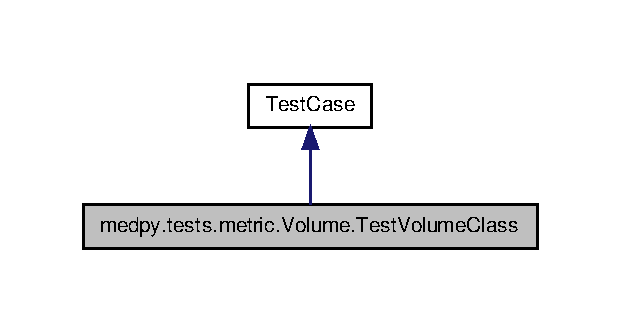
\includegraphics[width=298pt]{classmedpy_1_1tests_1_1metric_1_1Volume_1_1TestVolumeClass__inherit__graph}
\end{center}
\end{figure}


Collaboration diagram for medpy.tests.metric.Volume.TestVolumeClass:\nopagebreak
\begin{figure}[H]
\begin{center}
\leavevmode
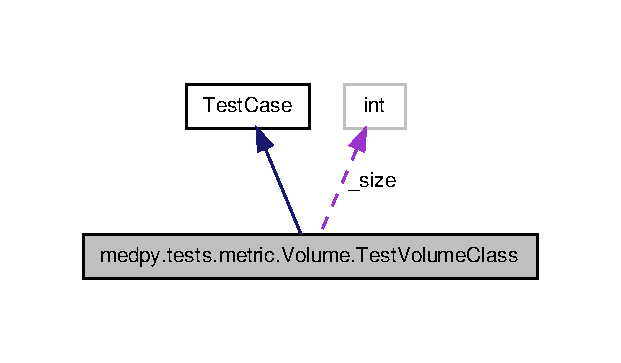
\includegraphics[width=298pt]{classmedpy_1_1tests_1_1metric_1_1Volume_1_1TestVolumeClass__coll__graph}
\end{center}
\end{figure}
\subsection*{Public Member Functions}
\begin{DoxyCompactItemize}
\item 
\hypertarget{classmedpy_1_1tests_1_1metric_1_1Volume_1_1TestVolumeClass_a6339b148e87a5b58312f90ae8afd6faa}{
def {\bfseries test\_\-GetVolumetricOverlapError}}
\label{classmedpy_1_1tests_1_1metric_1_1Volume_1_1TestVolumeClass_a6339b148e87a5b58312f90ae8afd6faa}

\item 
\hypertarget{classmedpy_1_1tests_1_1metric_1_1Volume_1_1TestVolumeClass_a071a3ee1de1a3dcab9e4644501c1b5aa}{
def {\bfseries test\_\-GetRelativeVolumeDifference}}
\label{classmedpy_1_1tests_1_1metric_1_1Volume_1_1TestVolumeClass_a071a3ee1de1a3dcab9e4644501c1b5aa}

\end{DoxyCompactItemize}
\subsection*{Private Member Functions}
\begin{DoxyCompactItemize}
\item 
def \hyperlink{classmedpy_1_1tests_1_1metric_1_1Volume_1_1TestVolumeClass_a23f94273ab3bf9772075a42a831210e4}{\_\-createTestImages}
\begin{DoxyCompactList}\small\item\em Creates some images used in the tests. \end{DoxyCompactList}\end{DoxyCompactItemize}
\subsection*{Static Private Attributes}
\begin{DoxyCompactItemize}
\item 
\hypertarget{classmedpy_1_1tests_1_1metric_1_1Volume_1_1TestVolumeClass_a44c8945493e1c3068fb8a0361bd2ce1a}{
int {\bfseries \_\-size} = 24}
\label{classmedpy_1_1tests_1_1metric_1_1Volume_1_1TestVolumeClass_a44c8945493e1c3068fb8a0361bd2ce1a}

\end{DoxyCompactItemize}


\subsection{Detailed Description}


Definition at line 23 of file Volume.py.



\subsection{Member Function Documentation}
\hypertarget{classmedpy_1_1tests_1_1metric_1_1Volume_1_1TestVolumeClass_a23f94273ab3bf9772075a42a831210e4}{
\index{medpy::tests::metric::Volume::TestVolumeClass@{medpy::tests::metric::Volume::TestVolumeClass}!\_\-createTestImages@{\_\-createTestImages}}
\index{\_\-createTestImages@{\_\-createTestImages}!medpy::tests::metric::Volume::TestVolumeClass@{medpy::tests::metric::Volume::TestVolumeClass}}
\subsubsection[{\_\-createTestImages}]{\setlength{\rightskip}{0pt plus 5cm}def medpy.tests.metric.Volume.TestVolumeClass.\_\-createTestImages (
\begin{DoxyParamCaption}
\item[{}]{self}
\end{DoxyParamCaption}
)\hspace{0.3cm}{\ttfamily  \mbox{[}private\mbox{]}}}}
\label{classmedpy_1_1tests_1_1metric_1_1Volume_1_1TestVolumeClass_a23f94273ab3bf9772075a42a831210e4}


Creates some images used in the tests. 



Definition at line 121 of file Volume.py.



The documentation for this class was generated from the following file:\begin{DoxyCompactItemize}
\item 
/home/loli/Programming/Python/MedPy/src/medpy/tests/metric/Volume.py\end{DoxyCompactItemize}

\hypertarget{classmedpy_1_1metric_1_1Volume_1_1Volume}{
\section{medpy.metric.Volume.Volume Class Reference}
\label{classmedpy_1_1metric_1_1Volume_1_1Volume}\index{medpy::metric::Volume::Volume@{medpy::metric::Volume::Volume}}
}


Computes different volume metrics between two 3D-\/images contain each a binary object.  




Inheritance diagram for medpy.metric.Volume.Volume:\nopagebreak
\begin{figure}[H]
\begin{center}
\leavevmode
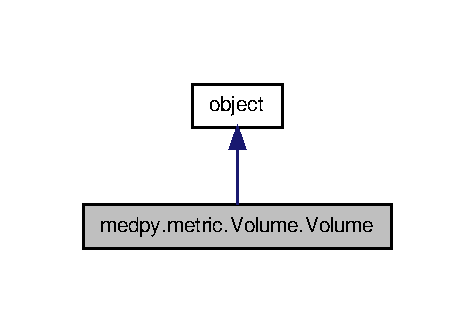
\includegraphics[width=228pt]{classmedpy_1_1metric_1_1Volume_1_1Volume__inherit__graph}
\end{center}
\end{figure}


Collaboration diagram for medpy.metric.Volume.Volume:\nopagebreak
\begin{figure}[H]
\begin{center}
\leavevmode
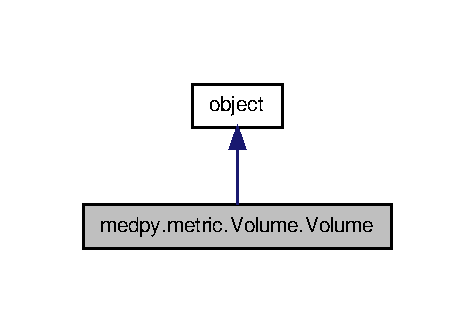
\includegraphics[width=228pt]{classmedpy_1_1metric_1_1Volume_1_1Volume__coll__graph}
\end{center}
\end{figure}
\subsection*{Public Member Functions}
\begin{DoxyCompactItemize}
\item 
def \hyperlink{classmedpy_1_1metric_1_1Volume_1_1Volume_acd9bb57619003117d40ddb45059f160d}{\_\-\_\-init\_\-\_\-}
\begin{DoxyCompactList}\small\item\em Initialize the class with two binary images whose 0 values are considered to be background voxels and the 1 values foreground. \end{DoxyCompactList}\item 
def \hyperlink{classmedpy_1_1metric_1_1Volume_1_1Volume_a0432d5eeea15c24f159ab0c7737be4ad}{GetRelativeVolumeDifference}
\begin{DoxyCompactList}\small\item\em Returns the relative volume difference between two shapes defined by the non-\/background voxels of in the binary images. \end{DoxyCompactList}\item 
def \hyperlink{classmedpy_1_1metric_1_1Volume_1_1Volume_ac9520b102a7355e1c3b1e6e7338f8d1d}{GetVolumetricOverlapError}
\begin{DoxyCompactList}\small\item\em Returns the volumetric overlap error between two shapes defined by the non-\/background voxels of in two binary images. \end{DoxyCompactList}\item 
\hypertarget{classmedpy_1_1metric_1_1Volume_1_1Volume_a2b74258c665afe8c9fb75d81539b2072}{
def \hyperlink{classmedpy_1_1metric_1_1Volume_1_1Volume_a2b74258c665afe8c9fb75d81539b2072}{GetMaskSize}}
\label{classmedpy_1_1metric_1_1Volume_1_1Volume_a2b74258c665afe8c9fb75d81539b2072}

\begin{DoxyCompactList}\small\item\em Computes the mask objects size if not yet done and returns it. \end{DoxyCompactList}\item 
\hypertarget{classmedpy_1_1metric_1_1Volume_1_1Volume_a9b83c53e0f5742f89e9e42fb91fde96f}{
def \hyperlink{classmedpy_1_1metric_1_1Volume_1_1Volume_a9b83c53e0f5742f89e9e42fb91fde96f}{GetReferenceSize}}
\label{classmedpy_1_1metric_1_1Volume_1_1Volume_a9b83c53e0f5742f89e9e42fb91fde96f}

\begin{DoxyCompactList}\small\item\em Computes the reference objects size if not yet done and returns it. \end{DoxyCompactList}\item 
\hypertarget{classmedpy_1_1metric_1_1Volume_1_1Volume_a675fe69a77ee67b93da82af7f138deaa}{
def \hyperlink{classmedpy_1_1metric_1_1Volume_1_1Volume_a675fe69a77ee67b93da82af7f138deaa}{GetIntersectionSize}}
\label{classmedpy_1_1metric_1_1Volume_1_1Volume_a675fe69a77ee67b93da82af7f138deaa}

\begin{DoxyCompactList}\small\item\em Computes the two objects intersection size if not yet done and returns it. \end{DoxyCompactList}\item 
\hypertarget{classmedpy_1_1metric_1_1Volume_1_1Volume_a2ba55a81e112ad5b40fc7d8f58e71f0d}{
def \hyperlink{classmedpy_1_1metric_1_1Volume_1_1Volume_a2ba55a81e112ad5b40fc7d8f58e71f0d}{GetUnionSize}}
\label{classmedpy_1_1metric_1_1Volume_1_1Volume_a2ba55a81e112ad5b40fc7d8f58e71f0d}

\begin{DoxyCompactList}\small\item\em Computes the two objects union size if not yet done and returns it. \end{DoxyCompactList}\end{DoxyCompactItemize}
\subsection*{Private Member Functions}
\begin{DoxyCompactItemize}
\item 
def \hyperlink{classmedpy_1_1metric_1_1Volume_1_1Volume_a30566577c9f3e1812da2c0ecc1e9543b}{\_\-ComputeIntersectionWindow}
\begin{DoxyCompactList}\small\item\em Computes and sets the intersection windows of the two images. \end{DoxyCompactList}\item 
\hypertarget{classmedpy_1_1metric_1_1Volume_1_1Volume_a28099a18f703f77e073e35d336da6db5}{
def \hyperlink{classmedpy_1_1metric_1_1Volume_1_1Volume_a28099a18f703f77e073e35d336da6db5}{\_\-ComputeUnionAndIntersection}}
\label{classmedpy_1_1metric_1_1Volume_1_1Volume_a28099a18f703f77e073e35d336da6db5}

\begin{DoxyCompactList}\small\item\em Computes and sets the two image shapes union and intersection sizes. \end{DoxyCompactList}\end{DoxyCompactItemize}
\subsection*{Static Private Attributes}
\begin{DoxyCompactItemize}
\item 
\hypertarget{classmedpy_1_1metric_1_1Volume_1_1Volume_a3437bb5928998234f90e917f295e9f1a}{
{\bfseries \_\-mask} = None}
\label{classmedpy_1_1metric_1_1Volume_1_1Volume_a3437bb5928998234f90e917f295e9f1a}

\item 
\hypertarget{classmedpy_1_1metric_1_1Volume_1_1Volume_ab6340306acf9010f924bee565c293a67}{
{\bfseries \_\-reference} = None}
\label{classmedpy_1_1metric_1_1Volume_1_1Volume_ab6340306acf9010f924bee565c293a67}

\item 
\hypertarget{classmedpy_1_1metric_1_1Volume_1_1Volume_a8e479ed7d6f62ea93684f0425d7c0876}{
{\bfseries \_\-mask\_\-offset} = None}
\label{classmedpy_1_1metric_1_1Volume_1_1Volume_a8e479ed7d6f62ea93684f0425d7c0876}

\item 
\hypertarget{classmedpy_1_1metric_1_1Volume_1_1Volume_aa1bb2b905b05ec2f7d0293e28cd377d2}{
{\bfseries \_\-reference\_\-offset} = None}
\label{classmedpy_1_1metric_1_1Volume_1_1Volume_aa1bb2b905b05ec2f7d0293e28cd377d2}

\item 
\hypertarget{classmedpy_1_1metric_1_1Volume_1_1Volume_a0da7280647425ce48e8bbba9f2eea751}{
{\bfseries \_\-intersection\_\-window} = None}
\label{classmedpy_1_1metric_1_1Volume_1_1Volume_a0da7280647425ce48e8bbba9f2eea751}

\item 
\hypertarget{classmedpy_1_1metric_1_1Volume_1_1Volume_aa87392dfe821aa7eed8973211fb54fdb}{
{\bfseries \_\-mask\_\-size} = None}
\label{classmedpy_1_1metric_1_1Volume_1_1Volume_aa87392dfe821aa7eed8973211fb54fdb}

\item 
\hypertarget{classmedpy_1_1metric_1_1Volume_1_1Volume_a6996e5b448ef3818964f409e36d7fea6}{
{\bfseries \_\-reference\_\-size} = None}
\label{classmedpy_1_1metric_1_1Volume_1_1Volume_a6996e5b448ef3818964f409e36d7fea6}

\item 
\hypertarget{classmedpy_1_1metric_1_1Volume_1_1Volume_af3427348038c6318d388eeee19dc303c}{
{\bfseries \_\-union\_\-size} = None}
\label{classmedpy_1_1metric_1_1Volume_1_1Volume_af3427348038c6318d388eeee19dc303c}

\item 
\hypertarget{classmedpy_1_1metric_1_1Volume_1_1Volume_a4d8bd483c09923985b8376b3a8850e86}{
{\bfseries \_\-intersection\_\-size} = None}
\label{classmedpy_1_1metric_1_1Volume_1_1Volume_a4d8bd483c09923985b8376b3a8850e86}

\end{DoxyCompactItemize}


\subsection{Detailed Description}
Computes different volume metrics between two 3D-\/images contain each a binary object. 

Beside this provides a number of statistics of the two images.

Metrics defined in: Heimann, T.; van Ginneken, B.; Styner, M.A.; Arzhaeva, Y.; Aurich, V.; Bauer, C.; Beck, A.; Becker, C.; Beichel, R.; Bekes, G.; Bello, F.; Binnig, G.; Bischof, H.; Bornik, A.; Cashman, P.; Ying Chi; Cordova, A.; Dawant, B.M.; Fidrich, M.; Furst, J.D.; Furukawa, D.; Grenacher, L.; Hornegger, J.; Kainmuller, D.; Kitney, R.I.; Kobatake, H.; Lamecker, H.; Lange, T.; Jeongjin Lee; Lennon, B.; Rui Li; Senhu Li; Meinzer, H.-\/P.; Nemeth, G.; Raicu, D.S.; Rau, A.-\/M.; van Rikxoort, E.M.; Rousson, M.; Rusko, L.; Saddi, K.A.; Schmidt, G.; Seghers, D.; Shimizu, A.; Slagmolen, P.; Sorantin, E.; Soza, G.; Susomboon, R.; Waite, J.M.; Wimmer, A.; Wolf, I.; , \char`\"{}Comparison and Evaluation of Methods for Liver Segmentation From CT Datasets,\char`\"{} Medical Imaging, IEEE Transactions on , vol.28, no.8, pp.1251-\/1265, Aug. 2009 doi: 10.1109/TMI.2009.2013851 \begin{DoxyVerb}The mask image as scipy array.\end{DoxyVerb}
 

Definition at line 32 of file Volume.py.



\subsection{Constructor \& Destructor Documentation}
\hypertarget{classmedpy_1_1metric_1_1Volume_1_1Volume_acd9bb57619003117d40ddb45059f160d}{
\index{medpy::metric::Volume::Volume@{medpy::metric::Volume::Volume}!\_\-\_\-init\_\-\_\-@{\_\-\_\-init\_\-\_\-}}
\index{\_\-\_\-init\_\-\_\-@{\_\-\_\-init\_\-\_\-}!medpy::metric::Volume::Volume@{medpy::metric::Volume::Volume}}
\subsubsection[{\_\-\_\-init\_\-\_\-}]{\setlength{\rightskip}{0pt plus 5cm}def medpy.metric.Volume.Volume.\_\-\_\-init\_\-\_\- (
\begin{DoxyParamCaption}
\item[{}]{self, }
\item[{}]{mask, }
\item[{}]{reference, }
\item[{}]{mask\_\-offset = {\ttfamily \mbox{[}0}, }
\item[{}]{reference\_\-offset = {\ttfamily \mbox{[}0}}
\end{DoxyParamCaption}
)}}
\label{classmedpy_1_1metric_1_1Volume_1_1Volume_acd9bb57619003117d40ddb45059f160d}


Initialize the class with two binary images whose 0 values are considered to be background voxels and the 1 values foreground. 


\begin{DoxyParams}{Parameters}
{\em mask,:} & mask as an scipy array (3D image) \\
\hline
{\em reference,:} & reference as an scipy array (3D image) \\
\hline
{\em mask\_\-offset,:} & offset of the mask array to 0,0,0-\/origin \\
\hline
{\em mask\_\-offset,:} & offset of the reference array to 0,0,0-\/origin \\
\hline
\end{DoxyParams}


Definition at line 62 of file Volume.py.



\subsection{Member Function Documentation}
\hypertarget{classmedpy_1_1metric_1_1Volume_1_1Volume_a30566577c9f3e1812da2c0ecc1e9543b}{
\index{medpy::metric::Volume::Volume@{medpy::metric::Volume::Volume}!\_\-ComputeIntersectionWindow@{\_\-ComputeIntersectionWindow}}
\index{\_\-ComputeIntersectionWindow@{\_\-ComputeIntersectionWindow}!medpy::metric::Volume::Volume@{medpy::metric::Volume::Volume}}
\subsubsection[{\_\-ComputeIntersectionWindow}]{\setlength{\rightskip}{0pt plus 5cm}def medpy.metric.Volume.Volume.\_\-ComputeIntersectionWindow (
\begin{DoxyParamCaption}
\item[{}]{self}
\end{DoxyParamCaption}
)\hspace{0.3cm}{\ttfamily  \mbox{[}private\mbox{]}}}}
\label{classmedpy_1_1metric_1_1Volume_1_1Volume_a30566577c9f3e1812da2c0ecc1e9543b}


Computes and sets the intersection windows of the two images. 

The intersection window marks the area in which the two images bounding boxes intersect. The returned rectangle is defined by its lower-\/left and upper-\/right corner. 

Definition at line 174 of file Volume.py.

\hypertarget{classmedpy_1_1metric_1_1Volume_1_1Volume_a0432d5eeea15c24f159ab0c7737be4ad}{
\index{medpy::metric::Volume::Volume@{medpy::metric::Volume::Volume}!GetRelativeVolumeDifference@{GetRelativeVolumeDifference}}
\index{GetRelativeVolumeDifference@{GetRelativeVolumeDifference}!medpy::metric::Volume::Volume@{medpy::metric::Volume::Volume}}
\subsubsection[{GetRelativeVolumeDifference}]{\setlength{\rightskip}{0pt plus 5cm}def medpy.metric.Volume.Volume.GetRelativeVolumeDifference (
\begin{DoxyParamCaption}
\item[{}]{self}
\end{DoxyParamCaption}
)}}
\label{classmedpy_1_1metric_1_1Volume_1_1Volume_a0432d5eeea15c24f159ab0c7737be4ad}


Returns the relative volume difference between two shapes defined by the non-\/background voxels of in the binary images. 

The relative volume distance of 0 means that the volumes are identical. Note that this doesn't apply that the shapes are identical or overlap at all. The result is given as signed number \mbox{[}-\/100,+100\mbox{]} to indicate over-\/ or under-\/segmentation. Warning: Can produce values greater than -\//+100 if the difference in volume exceeds 50\%. Positive values means that the mask volume is too big, a negative value that it is too small.

Warning: This measure is not actually a metric, as it is not symmetric.

Metric definition: The relative volume difference between two sets of voxels $S(A)$ and $S(b)$ is given in percent and defined as: \[ 100 * \frac{|A - B|}{|B|} \] 

Definition at line 93 of file Volume.py.

\hypertarget{classmedpy_1_1metric_1_1Volume_1_1Volume_ac9520b102a7355e1c3b1e6e7338f8d1d}{
\index{medpy::metric::Volume::Volume@{medpy::metric::Volume::Volume}!GetVolumetricOverlapError@{GetVolumetricOverlapError}}
\index{GetVolumetricOverlapError@{GetVolumetricOverlapError}!medpy::metric::Volume::Volume@{medpy::metric::Volume::Volume}}
\subsubsection[{GetVolumetricOverlapError}]{\setlength{\rightskip}{0pt plus 5cm}def medpy.metric.Volume.Volume.GetVolumetricOverlapError (
\begin{DoxyParamCaption}
\item[{}]{self}
\end{DoxyParamCaption}
)}}
\label{classmedpy_1_1metric_1_1Volume_1_1Volume_ac9520b102a7355e1c3b1e6e7338f8d1d}


Returns the volumetric overlap error between two shapes defined by the non-\/background voxels of in two binary images. 

The volumetric overlap error is 0 for a perfect match and 100 if the two shapes don't overlap at all.

Metric definition: The volumetric overlap error between two sets of voxels $S(A)$ and $S(b)$ is given in percent and defined as: \[ 100 * \left( 1 - \frac{|A\cap B|}{|A\cup B|} \right) \] 

Definition at line 118 of file Volume.py.



The documentation for this class was generated from the following file:\begin{DoxyCompactItemize}
\item 
/home/loli/Programming/Python/MedPy/src/medpy/metric/Volume.py\end{DoxyCompactItemize}

\hypertarget{classmedpy_1_1filter_1_1Watershed_1_1Watershed}{
\section{medpy.filter.Watershed.Watershed Class Reference}
\label{classmedpy_1_1filter_1_1Watershed_1_1Watershed}\index{medpy::filter::Watershed::Watershed@{medpy::filter::Watershed::Watershed}}
}


Inheritance diagram for medpy.filter.Watershed.Watershed:\nopagebreak
\begin{figure}[H]
\begin{center}
\leavevmode
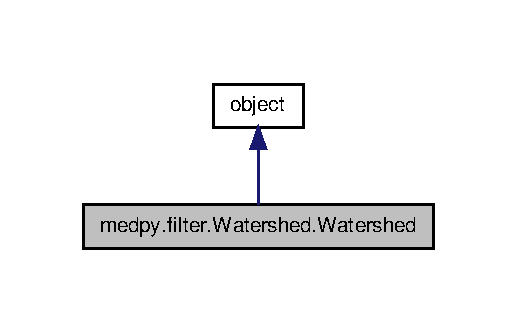
\includegraphics[width=248pt]{classmedpy_1_1filter_1_1Watershed_1_1Watershed__inherit__graph}
\end{center}
\end{figure}


Collaboration diagram for medpy.filter.Watershed.Watershed:\nopagebreak
\begin{figure}[H]
\begin{center}
\leavevmode
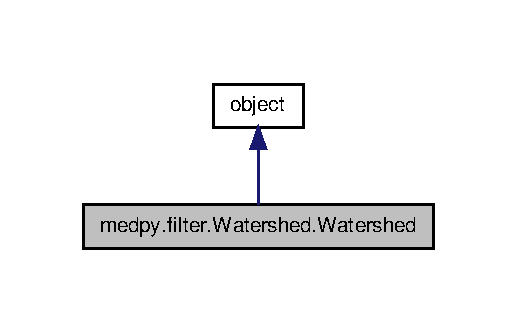
\includegraphics[width=248pt]{classmedpy_1_1filter_1_1Watershed_1_1Watershed__coll__graph}
\end{center}
\end{figure}


\subsection{Detailed Description}


Definition at line 22 of file Watershed.py.



The documentation for this class was generated from the following file:\begin{DoxyCompactItemize}
\item 
/home/loli/Programming/Python/MedPy/src/medpy/filter/Watershed.py\end{DoxyCompactItemize}

\printindex
\end{document}
